Ten rozdział prezentuje wyniki przeprowadzonego eksperymentu, koncentrując się
na uzyskanych danych i efektach badania.
Zawiera zarówno surowe dane, jak i ich znormalizowaną wersję, a także
statystyczne porównanie obu grup.
W końcowej części przeprowadzona zostaje analiza z wykorzystaniem testu
t~Welcha w celu weryfikacji hipotezy zerowej \(H_{0}\).


\section{Uzyskane pomiary}

Od października do listopada 2024 roku autor pracy przeprowadził 10
eksperymentów z udziałem zgłoszonych do badania programistów.
Wszyscy uczestnicy ukończyli oba zadania.

Tabela~\ref{tab:czas_norm} przedstawia wykonane pomiary wraz ze znormalizowaną
wartością, normalizacja została szczegółowo opisana
w~podrozdziale~\ref{subsec:zmienne}.

\begin{table}[h]
    \centering
    \begin{tabular}{l|l|l|l|l}
        Grupa & Badany \(i\) & \(T_{1}(i) [s]\) & \(T_{2}(i) [s]\) &
        \(T_2^{norm}(i) = \frac{T_{2}(i)}{T_{1}(i)}\) \\\hline\hline
        \multirow{5}{*}{1} & \underline{1} & 2027 & 529 & 0,2604834 \\
        & \underline{2} & 1720 & 180 & 0,1046511 \\
        & 3             & 1106 & 300 & 0,2712477 \\
        & \underline{4} & 2265 & 273 & 0,1205298 \\
        & 5             & 380  & 70  & 0,1842105 \\ \hline
        \multirow{5}{*}{2} & \underline{6} & 2031 & 581 & 0,2860659 \\
        & 7             & 411  & 120 & 0,2919708 \\
        & \underline{8} & 2017 & 670 & 0,3321765 \\
        & \underline{9} & 1213 & 480 & 0,3957131 \\
        & 10            & 221  & 523 & 2,3665158 \\ \hline
    \end{tabular}
    \caption{\label{tab:czas_norm}Pomiary wykonane podczas eksperymentów.}
\end{table}

\begin{table}[h]
    \centering
    \begin{tabular}{l|l|l|l|l|l}
        Grupa & Badany \(i\) & Doświadczenie Java [lata] & Technologia & Wykształcenie & Dziedzina
        \\ \hline\hline
        \multirow{5}{*}{1} & \underline{1} & 2 & Spring & mgr & Bankowość
        \\
        & \underline{2} & 3  & Spring & mgr       & Linie lotnicze      \\
        & 3             & 7  & Spring & mgr       & Bankowość           \\
        & \underline{4} & 20 & Spring & mgr       & Bankowość           \\
        & 5             & 9  & EJB    & kurs      & Handel              \\ \hline
        \multirow{5}{*}{2} & \underline{6} & 5 & Spring & mgr & Bankowość
        \\
        & 7             & 20 & Spring & mgr       & Bankowość           \\
        & \underline{8} & 5  & Spring & kurs      & Bankowość           \\
        & \underline{9} & 2  & Go     & technikum & Transport/Produkcja \\
        & 10            & 3  & Spring & mgr       & Biofarmaceutyka     \\ \hline
    \end{tabular}
    \caption{\label{tab:demografia}Doświadczenie, aktualnie używana technologia i dziedzina,
        którą zajmują się badani programiści}
\end{table}

Jako dodatkowa obserwacja, w 6 przypadkach (podkreślonych w
tabeli~\ref{tab:czas_norm}) eksperyment trwał dłużej niż założone 45 minut, ale
nie dużej niż godzinę.
Świadczy to o niedoszacowanej estymacji trwania badania przez autora pracy ---
czas badania powinien zostać ustalony na 60 minut, aby poprawnie odzwierciedlić
oczekiwania czasowe wobec badanych.

\subsection{Odrzuczenie próbki}

Uczestnik badania \(i = 10\) wykonał zadanie poprawnie, ale ---
w przekonaniu prowadzącego eksperyment --- nie zrozumiał poprawnie zadania
drugiego, wykonał implementację, która nie dotyczyła testu, a to spowodowało
nieadekwatnie dłuższy czas.
Wobec czego założenie, że w czasie wykonania zadania pierwszego zawiera się
czytanie i zrozumienie kodu, nie miało w tym przypadku zastosowania.
W związku z tym uznaje się, że ten eksperyment zakończył się niepowodzeniem,
nie dostarczając danych zgodnie z poczynionym założeniem.
Nie przewidziano takiego przypadku w zaprojektowaniu eksperymentu.
Tę próbkę autor pracy zdecydował się odrzucić z dalszej analizy statystycznej.

\section{Statystyczna analiza danych}

\begin{figure}[h]
    \centering 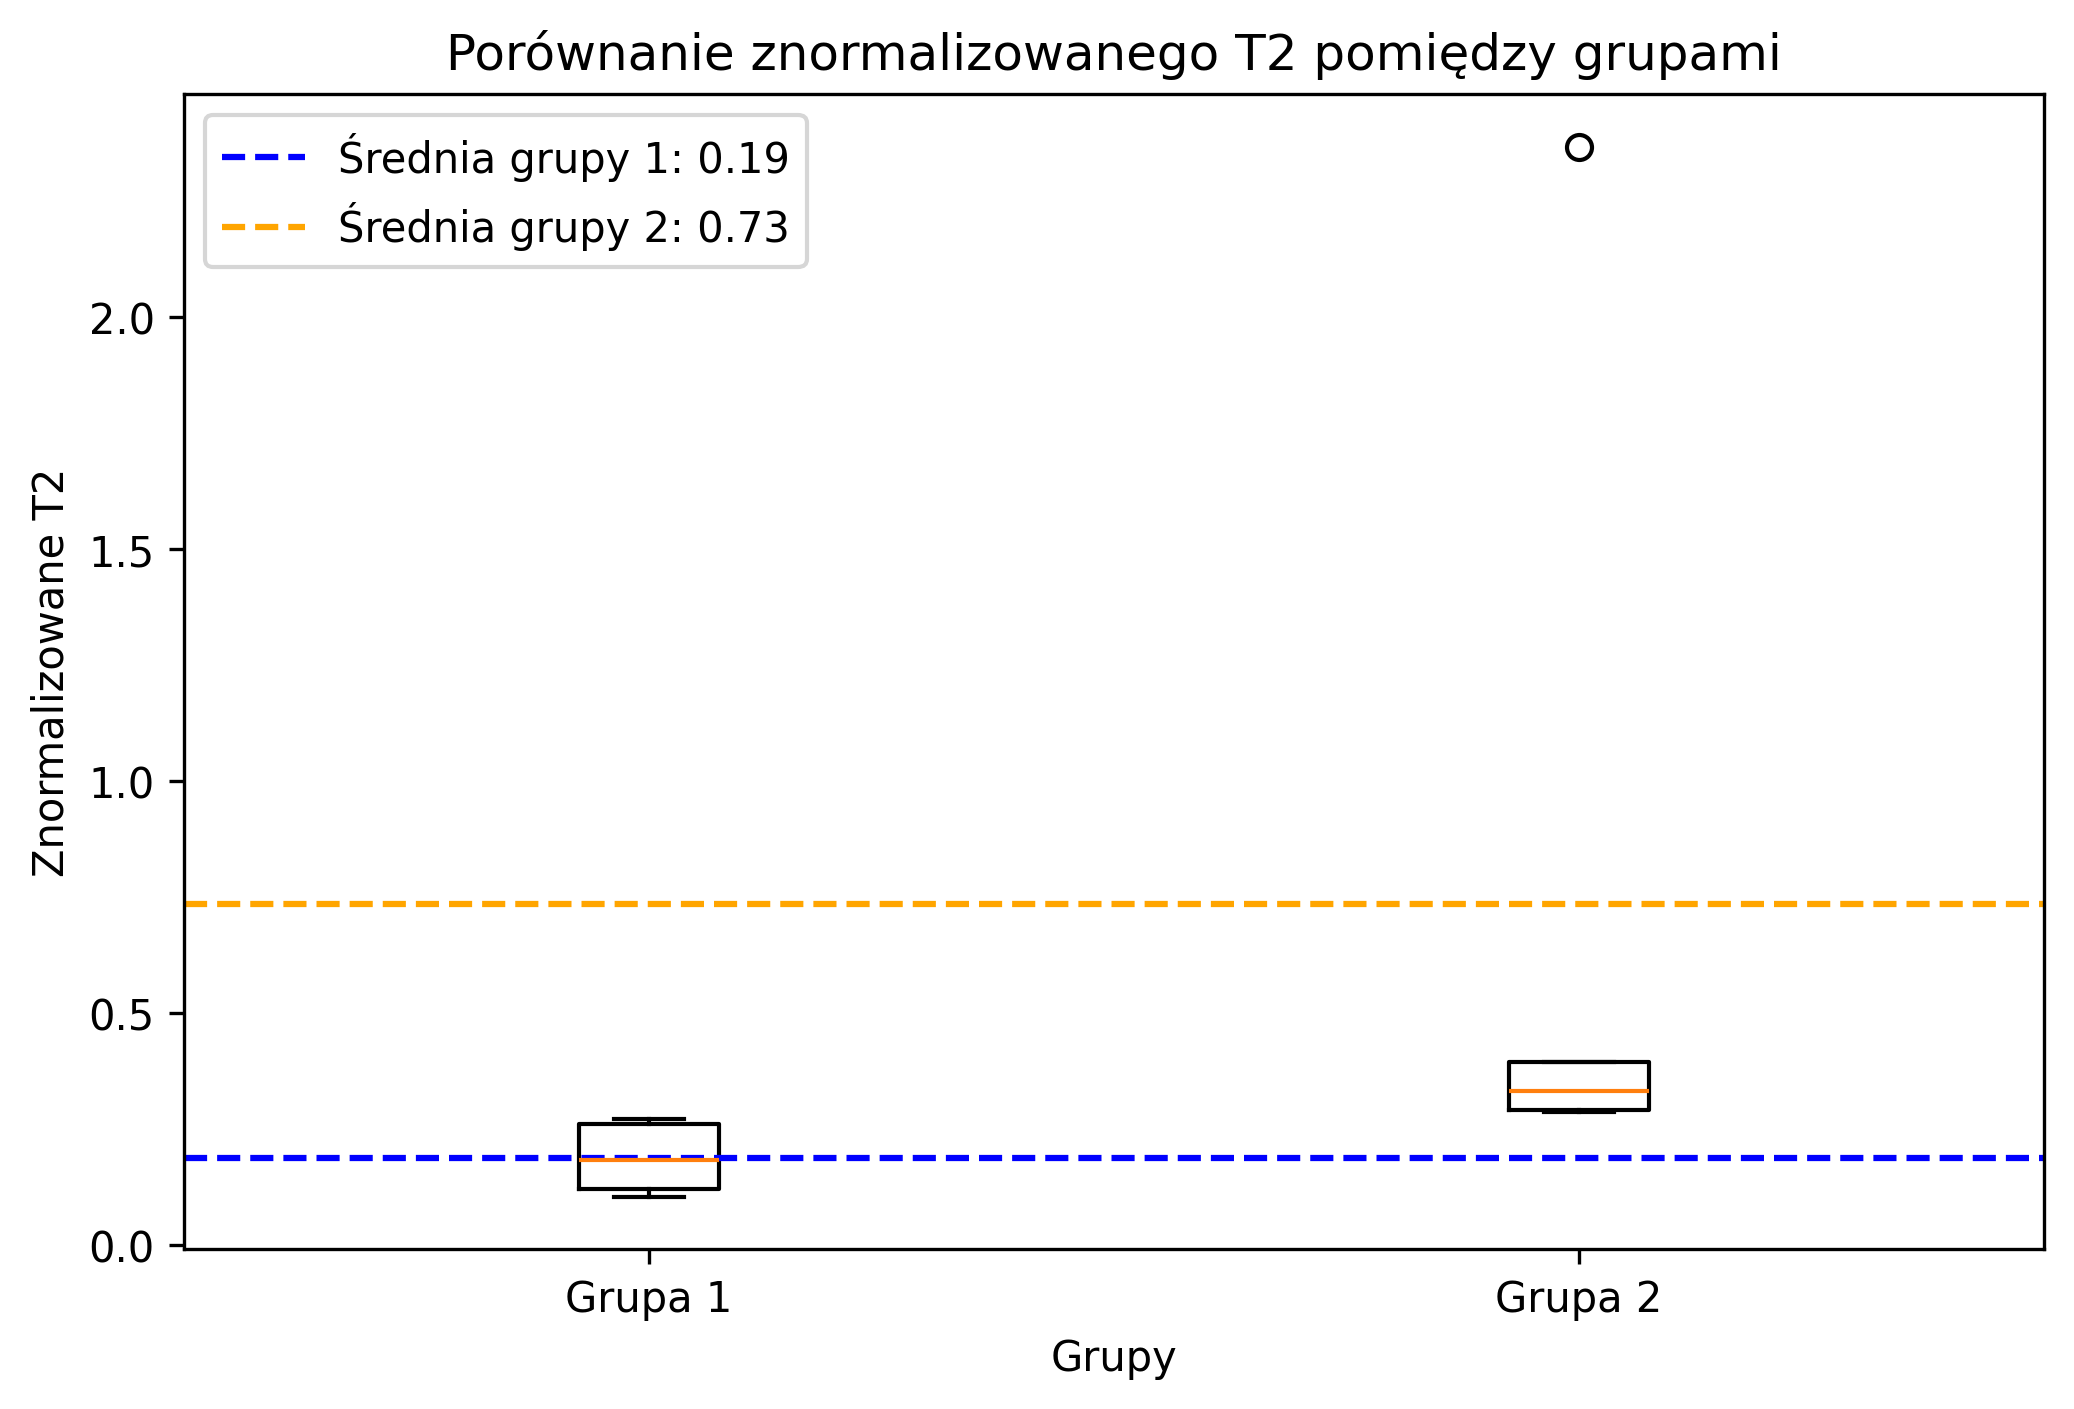
\includegraphics[width=0.8\linewidth]{diagramy/normalized_time_comparison}
    \caption{Wykres pudełkowy wyników obu grup}
    \label{fig:results_stats}
\end{figure}

Na Rysunku~\ref{fig:results_stats} przedstawiono wykres pudełkowy podsumowujący
pozyskane próbki.
Tabela~\ref{tab:wyniki_statystyka} przedstawia podstawowe wartości statystyczne.
Średnia grupy 2 jest o 74\% większa niż grupy 1.

\begin{table}[h]
    \centering
    \begin{tabular}{l|l|l|l|l|l}
        Grupa & Odchylenie standardowe & Średnia & Mediana & 25.\@ percentyl & 75.\@ percentyl \\ \hline \hline
        1 & 0.068 & 0.19 & 0.18 & 0.12 & 0.26 \\
        2 & 0.044 & 0.33 & 0.31 & 0.29 & 0.35 \\
    \end{tabular}
    \caption{\label{tab:wyniki_statystyka}Odchylenie standardowe, średnia, mediana, 25-ty i 75-ty percentyl w badanych grupach}
\end{table}

\section{Testowanie \(H_{0}\) t testem Welcha}

Test przeprowadzono przekazując zmierzone wartości \(T_{1}(i)\) i \(T_{2}(i)\),
następnie określając znormalizowaną wartość \((T_2^{norm}(i)\)otrzymując dwa
zbiory odpowiednie grupom.
Do funkcji przeprowadzającej t test \texttt{ttest\_ind} z biblioteki
\texttt{scipy.stats}~\cite{gonccalves2023effect} wprowadzono oba zbiory i
przetestowano, korzystając z parametrów uruchamiających t~test Welcha.

\lstinputlisting[language=Python,
    caption=\lstname,
    label={lst:ttest}]{ttest.py}

Wynikiem skryptu jest wydruk na standardowe wyjście przedstawione na Listingu~\ref{lst:ttest_output}.

\begin{lstlisting}[caption={Standardowe wyjście skryptu \texttt{ttest.py}},
    label={lst:ttest_output}]
First group seconds normalized: [0.2604834731129748, 0.10465116279069768, 0.27124773960216997, 0.1205298013245033, 0.18421052631578946]
Second group seconds normalized: [0.2860659773510586, 0.291970802919708, 0.3321764997521071, 0.3957131079967024]
First group mean: 0.18822454062922706
Second group mean: 0.32648159700489404
t value: -3.2386981867032234
p value: 0.01478208258587689
\end{lstlisting}

Dla potwierdzenia poprawności wprowadzonych danych można porównać wartości obu
grup \texttt{group normalized} z wydruku z danymi z Tabeli~\ref{tab:czas_norm}.
Wynikiem testu t Welcha jest wartość \(t = -3,23\) z \(p = 0,0148\).

Taka wartość \(t\) wskazuje, że wynik jest około 3,23-krotnie większy niż standardowy
błąd różnicy, co wskazuje na znaczną i statystycznie istotną różnicę pomiędzy
grupami.
Jednocześnie określa, że grupa rozwiązująca zadanie oparte o kod źródłowy o
niższym stopniu sprzężenia szybciej rozwiązała zadanie drugie.

\begin{figure}[h]
    \centering 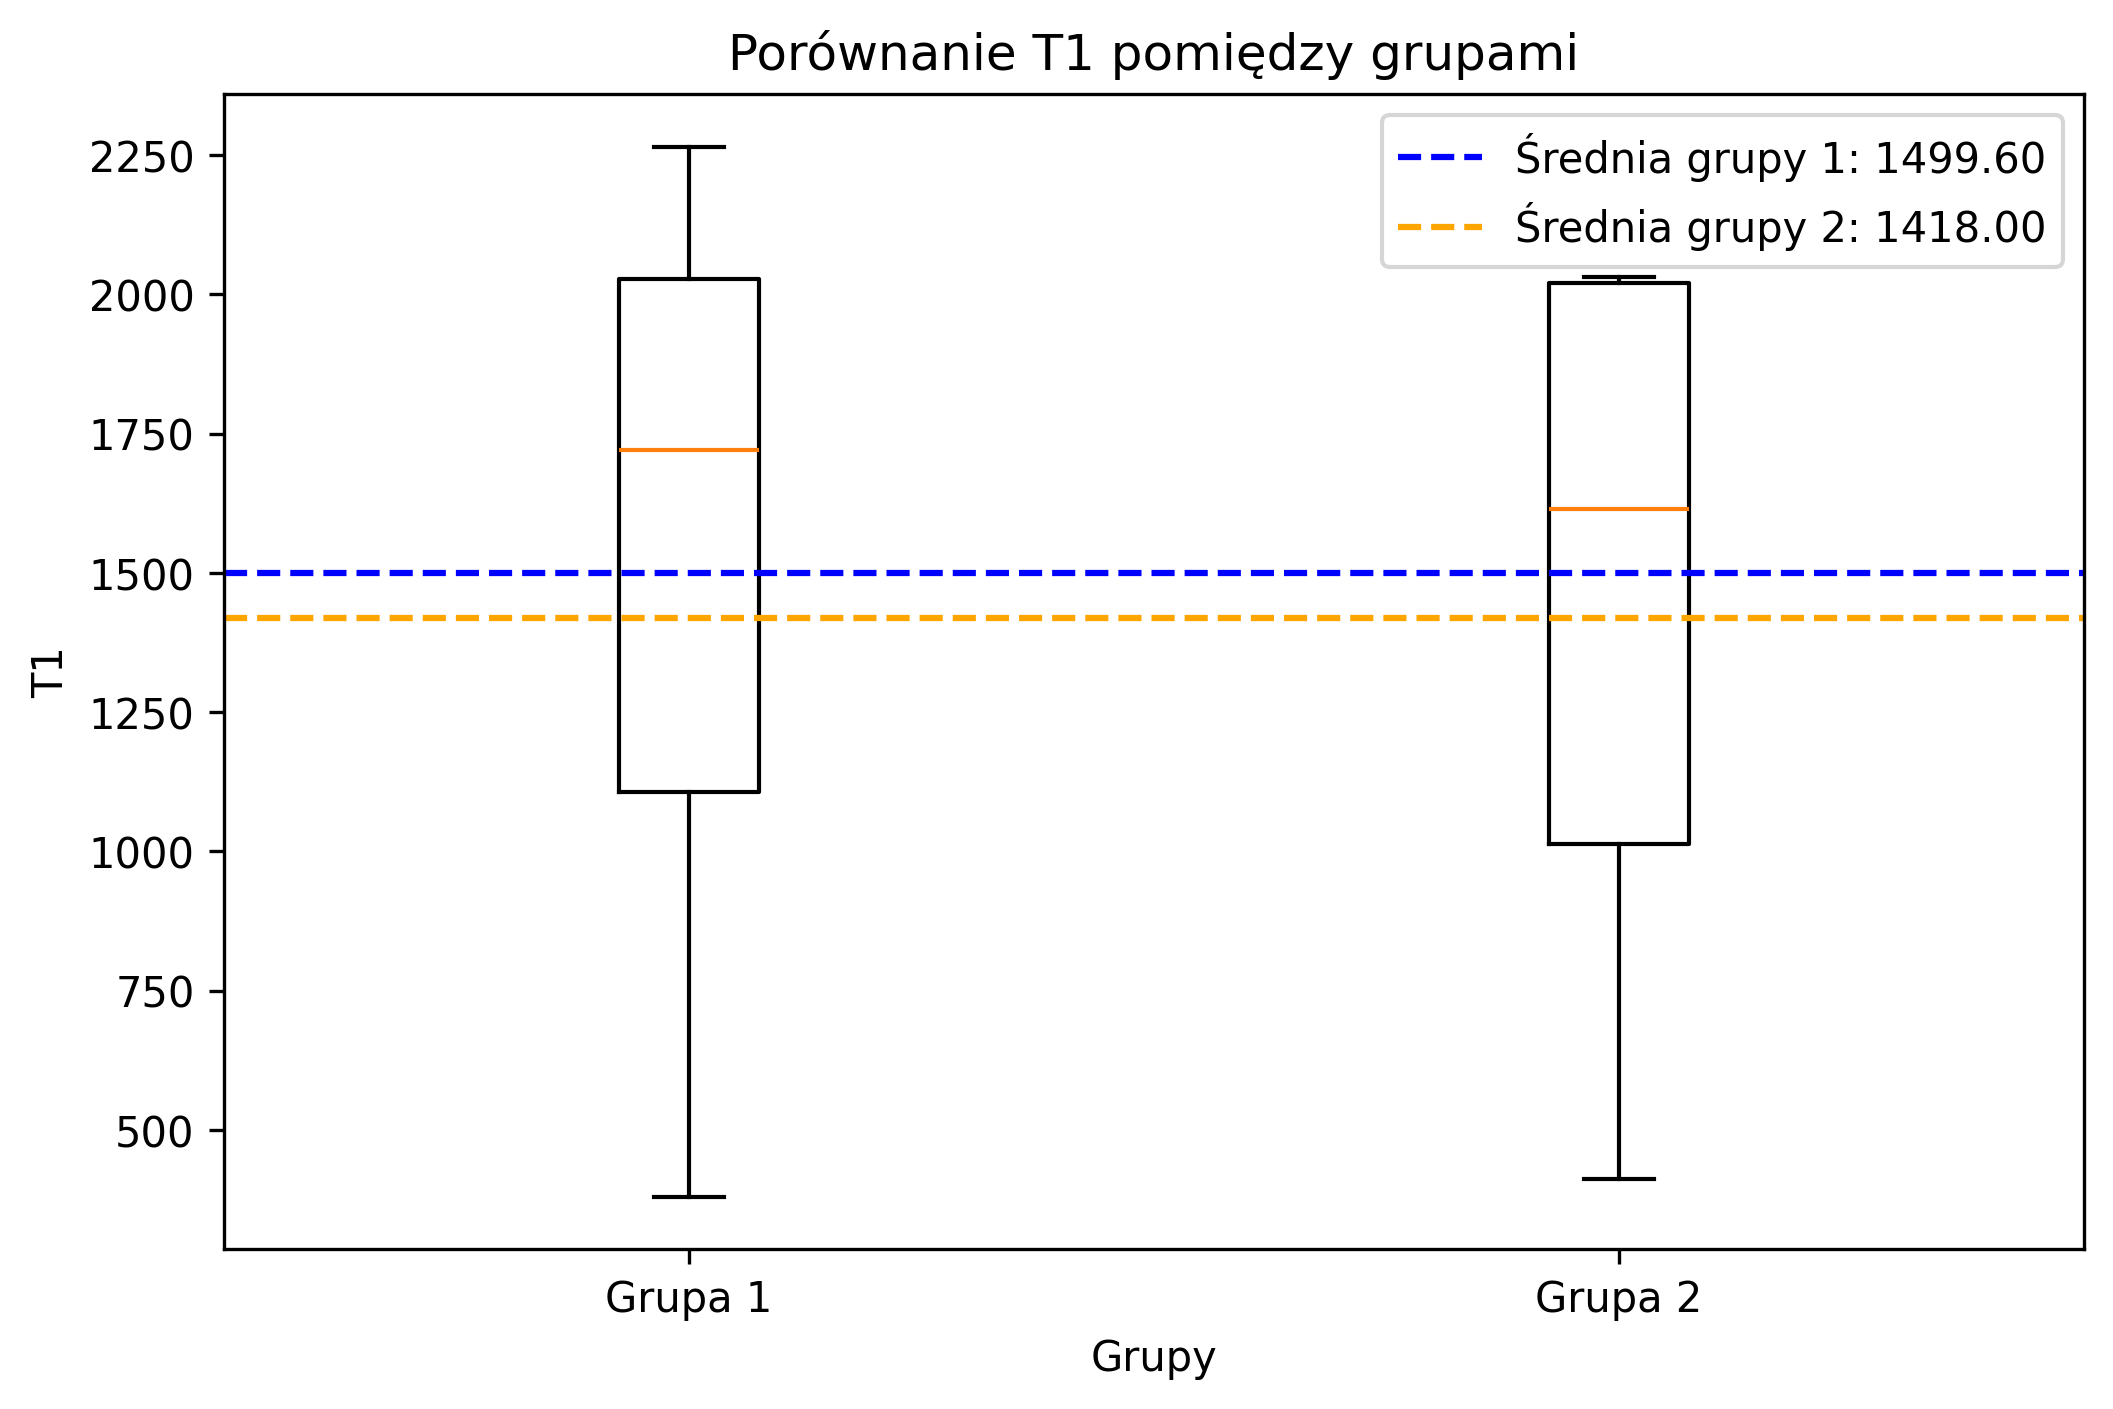
\includegraphics[width=0.7\linewidth]{diagramy/normalized_time_comparison_first}
    \caption{Wykres pudełkowy czasu \(T_{1}\) dla obu grup}
    \label{fig:results_first_status}
\end{figure}

Dodatkowo warto zbadać różnice w grupach pomiędzy czasem wykonywania zadania
kontrolnego --- określonego czasem \(T_{1}\).
Jeżeli różnica czasów jest statystycznie istotna w grupach, oznaczałoby to, że
stopień sprzężenia pomiędzy klasami ma wpływ na zadanie z pozoru niedotyczące
obszaru i należy odrzucić cały eksperyment ze względu na brak potwierdzenia
podstawowego założenia.
Wykres~\ref{fig:results_first_status} przedstawia różnice czasu w obu grupach.
Test t Welcha w tym przypadku daje wartości \(t = 0,15\) i \(p = 0.87\) co
wskazuje, że różnice są statystycznie nieistotne, zatem czas wykonania zadania
kontrolnego nie różni się statystycznie pomiędzy grupami eksperymentu.

\begin{table}[h]
    \centering
    \begin{tabular}{l|l|l|l|l|l}
        Grupa & odchylenie standardowe & średnia & mediana & 25 percentyl & 75 percentyl \\ \hline \hline
        1 & 681.32 & 1499.6 & 1720.0 & 1106.0 & 2027.0 \\
        2 & 669.07 & 1418.0 & 1615.0 & 1012.5 & 2020.5 \\
    \end{tabular}
    \caption{\label{tab:wyniki_zadanie_pierwszestatystyka}
    Odchylenie standardowe,\
        średnia, mediana, 25-ty i 75-ty percentyl dla czasu wykonania zadania \
        kontrolnego w badanych grupach}
\end{table}

Przy założeniu, że \(p < 0.05\) jest wymagane do odrzucenia hipotezy zerowej
\(H_{0}\), w świetle przeprowadzonego testu należy ją odrzucić, tym samym
dane uzyskane eksperymentalnie świadczą o statystycznie istotnej zależności
pomiędzy stopniem sprzężenia klasy i czasem wprowadzenia zmian w jej kodzie.

\section{Podsumowanie}

W toku eksperymentu pozyskano 10 próbek, z czego jedną należało odrzucić
ze względu na brak spełnienia założenia o zapoznaniu się z kodem źródłowym
podczas wykonywania zadania kontrolnego.

Uzyskane wyniki potwierdzają założenie, że czas wykonania zadania kontrolnego
w obu grupach nie różni się.
W związku z tym, nie ma podstaw do odrzucenia eksperymentu z powodu założenia,
że zadanie kontrolne jest wykonywane w obszarze wspólnym dla obu wariantów
programu.

Wartości \(T_{2}^{norm}\) są statystycznie różne dla obu grup, a ich średnia
różni się o \(74\%\).

W związku z tym eksperyment dostarczył wyników, które pozwalają na odrzucenie
hipotezy zerowej \(H_{0}\) i przyjęcie hipotezy \(H_{1}\), która głosi występowanie
statystycznie istotnej różnicy czasu wprowadzania zmian pomiędzy tożsamymi
programami o różnym stopniu sprzężenia.
Dodatkowo uzyskane dane pozwalają stwierdzić, że czas ten jest wyższy dla programów
o wyższym stopniu sprzężenia.

Z powyższych informacji można wyciągnąć wnioski co do zaprojektowania eksperymentu,
użytecznych heurystyk dla praktyków inżynierii oprogramowania, a także dalszych badań
w tym wąskim obszarze wpływu struktury programu obiektowego na koszty jego utrzymania.
